\documentclass[11pt]{article}

\usepackage[utf8]{inputenc}
\usepackage[margin=0.8in]{geometry}
\usepackage{graphicx}
\graphicspath{{img/}}
\usepackage{float}
\usepackage{amsmath}
\usepackage{amssymb}
\usepackage{setspace}
\usepackage{enumitem}
\usepackage{titlesec}
\usepackage{siunitx}
\usepackage[hidelinks]{hyperref}
\usepackage{comment}
\usepackage{caption}
\usepackage{gensymb}

\newenvironment{tight_enumerate}{
    \begin{enumerate}[label=(\alph*)]
    \setlength{\itemsep}{3pt}
    \setlength{\parskip}{0pt}}
    {\end{enumerate}}
\DeclareSIUnit{\msun}{
    \text{$M_{\odot}$}
}

\titleformat*{\section}{\large\bfseries}
\titleformat*{\subsection}{\normalsize\bfseries}

\title{\vspace{-3em} \textbf{Homework 3}}
\author{Justin Kang \\ AST 381: Star Formation}
\date{\vspace{-0.75em} October 17, 2018}

\begin{document}
\maketitle
\singlespacing
\pagenumbering{gobble}
\sloppy



\vspace{-2.5em}
\section*{Problem 1. Altogether Now: GMCs, Clusters, Protostars, and Outflow Feedback}
Consider a collapsing protostellar core that delivers mass to an accretion disk at its center at a constant rate $\dot{M}$. A fraction $f$ of the mass that reaches the disk is ejected in an outflow, and the remainder goes onto a protostar at the center of the disk. The material ejected in the outflow is launched at a velocity equal to the escape speed from the stellar surface. The protostar has a constant radius $R_{*}$ as it grows.
\begin{tight_enumerate}
\item Compute the momentum per unit stellar mass ejected by the outflow in the process of forming a star of final mass $M_{*}$. Evaluate this numerically for $f = 0.1$, $M_{*} = 0.5\ \si{\msun}$, and $R_{*} = 3\ R_{\odot}$. 

\item The material ejected into the outflow will shock and radiate energy as it interacts with the surrounding gas, so on large scales the outflow will conserve momentum rather than energy. The terminal velocity of the outflow material will be roughly the turbulent velocity dispersion $\sigma$ of the ambient cloud. If this cloud is forming a cluster of stars, all of mass $M_{*}$, with a constant star formation rate $\dot{M}_{cluster}$, compute the rate at which outflows inject kinetic energy into the cloud.

\item Suppose the cloud obeys Larson's relations, so its velocity dispersion, mass $M$, and size $L$ are related by $\sigma = 0.72(L/\si{pc})^{1/2}\ \si{km/s}$ and $M = 100(L/\si{pc})^{2}\ \si{\msun}$. Assuming the turbulence in the cloud decays at a rate what star formation rate is required for energy injected by outflows to balance the energy lost via the decay of turbulence? Evaluate this numerically for $L = 1$, $10$, and $100$ \si{pc}.

\item If stars form at the rate required to maintain the turbulence, what fraction of the cloud mass must be converted into stars per cloud free-fall time? Assume the cloud density is $\rho = M/L^{3}$. Again, evaluate numerically for $L = 1$, $10$, and $100$ \si{pc}. Are these numbers reasonable? Conversely, for what size clouds, if any, is it reasonable to neglect the energy injected by protostellar outflows?
\end{tight_enumerate}


\subsection*{Solution 1}
\begin{tight_enumerate}
\item We know that the outflow has a mass ejection rate of $f\dot{M}$, and the mass ejected at time $t$ does so at a velocity $v_{esc} = \sqrt{\frac{2GM(t)}{R_{*}}}$, where $M(t) = (1-f)\dot{M}t$ is the mass of the protostar at time $t$ (here we assume that $M = 0$ at $t = 0$, which is not physical). Given that the star will have a final mass of $M_{*}$, the time that this occurs is given by $t_{f} = \frac{M_{*}}{(1-f)\dot{M}}$. To find the momentum ejected by the outflow, we expand the following equation:
\begin{alignat*}{2}
p = &\int_{0}^{t_{f}}f\dot{M}\sqrt{\frac{2GM(t)}{R_{*}}}dt\ &=\ &\int_{0}^{t_{f}}f\dot{M}\sqrt{\frac{2G(1-f)\dot{M}t}{R_{*}}}dt \\
  = &\frac{2}{3}f\dot{M}\sqrt{\frac{2G(1-f)\dot{M}}{R_{*}}}t_{f}^{3/2}\ &=\ &\frac{2}{3}f\dot{M}^{3/2}\sqrt{\frac{2G}{R_{*}}}\sqrt{1-f}\left[\frac{M_{*}}{(1-f)\dot{M}}\right]^{3/2} \\
  = &\frac{2}{3}\frac{f}{1-f}M_{*}\sqrt{\frac{2GM_{*}}{R_{*}}}
\end{alignat*}
To convert this to momentum per unit stellar mass, we simply divide by $M_{*}$.\\
\fbox{$\therefore$ $\frac{p}{M_{*}} = \frac{2}{3}\frac{f}{1-f}\sqrt{\frac{2GM_{*}}{R_{*}}}$}\\
Plugging in $f = 0.1$, $M_{*} = 0.5\ \si{\msun}$, and $R_{*} = 3\ R_{\odot}$, $\frac{p}{M_{*}} = 18.679\ \si{km/s}$.

\item The initial momentum of material ejected in an outflow from a single star star is given by $p = \frac{2}{3}\frac{f}{1-f}M_{*}\sqrt{\frac{2GM_{*}}{R_{*}}}$. The final mass of the material ejected by the outflow is then this initial momentum divided by the terminal velocity. This is given by $M = \frac{p}{\sigma} = \frac{2}{3}\frac{f}{1-f}\frac{M_{*}}{\sigma}\sqrt{\frac{2GM_{*}}{R_{*}}}$. The kinetic energy injected by outflows from a single star is then given by $\frac{1}{2}M\sigma^{2}$. The cloud forms stars at a constant rate $\dot{M}_{cluster} \equiv M_{*}\dot{N}$, where $\dot{N}$ is the number rate of star formation, thus the rate at which outflows inject kinetic energy into the cloud will be given by this star formation number rate multiplied by the amount of kinetic energy injected by a single star.\\
\fbox{$\therefore$ the kinetic energy injection rate is given by $\frac{1}{3}\frac{f}{1-f}\dot{M}_{cluster}\sigma\sqrt{\frac{2GM_{*}}{R_{*}}}$.}

\item Assume that the decay time of turbulence is given by the eddy turnover time (the time it takes for an eddy to pass all of its energy to smaller scales, approximated as one revolution), $t = \frac{L}{\sigma}$. Suppose that the cloud loses its kinetic energy, $\frac{1}{2}M(\sqrt{3}\sigma)^{2}$, via turbulence within one decay time. The rate of energy loss is then given by $\frac{3}{2}M\sigma^{3}L^{-1}$. We can equate this to our energy injection rate from (b) to find the appropriate $\dot{M}_{cluster}$ to balance the energy injection and decay. After some algebra, this turns out to be 
\[\dot{M}_{cluster} = \frac{9}{2}\frac{1-f}{f}\frac{M\sigma^{2}}{L}\sqrt{\frac{R_{*}}{2GM_{*}}}\]
From Larson's relations, we can substitute for $\sigma$ and $M$. This ges us 
\[\dot{M}_{cluster} = 233.28\frac{1-f}{f}\sqrt{\frac{R_{*}}{2GM_{*}}}\frac{1}{L}\left(\frac{L}{\si{pc}}\right)^{3}\ \si{\msun.km^{2}/s^{2}}.\]
The star formation rate needed to balance the energy loss is tabulated below for the different lengths. Here we assume $f = 0.1$, $M_{*} = 0.5\ \si{\msun}$, and $R_{*} = 3\ R_{\odot}$.
\begin{table}[H]
\centering
\begin{tabular}{|c|c|}
\hline
Size of cloud (\si{pc}) & Star formation rate (\si{\msun/year}) \\
\hline
$1$ & $8.509\times10^{-6}$ \\
$10$ & $8.509\times10^{-4}$ \\
$100$ & $0.08509$ \\
\hline
\end{tabular}
\end{table}

\item The cloud free fall time is given by $t_{\text{ff}} = \sqrt{\frac{3\pi}{32G\rho}} = \sqrt{\frac{3{\pi}L^{3}}{32GM}}$. The mass fraction is then the total amount of mass used up in star formation in a free fall time divided by the total mass. Mathematically, this is given by $f_{*} = \frac{\dot{M}_{cluster}t_{\text{ff}}}{M}$. Plugging in our value for $\dot{M}_{cluster}$ from (c), 
\begin{align*}
f_{*} &= 233.28\frac{1-f}{f}\sqrt{\frac{3{\pi}L^{3}}{32GM}}\sqrt{\frac{R_{*}}{2GM_{*}}}\frac{1}{ML}\left(\frac{L}{\si{pc}}\right)^{3}\ \si{\msun.km^{2}/s^{2}} \\
&= 0.23328\frac{1-f}{f}\sqrt{\frac{3{\pi}L}{32G\si{\msun}}}\sqrt{\frac{R_{*}}{2GM_{*}}}\ \si{km^{2}/s^{2}}.
\end{align*}
The stellar mass fraction of the cloud is tabulated below for the different lengths. Here we assume $f = 0.1$, $M_{*} = 0.5\ \si{\msun}$, and $R_{*} = 3\ R_{\odot}$.
\begin{table}[H]
\centering
\begin{tabular}{|c|c|}
\hline
Size of cloud (\si{pc}) & Stellar mass fraction of cloud \\
\hline
$1$ & $0.0689$ \\
$10$ & $0.2179$ \\
$100$ & $0.689$ \\
\hline
\end{tabular}
\caption*{}
\end{table}
The first two numbers are reasonable, given that we observe a star formation efficiency on the order of $10\%$ for molecular clouds. However, the $68.9\%$ we calculate for the $100$ \si{pc} cloud is unphysical. As suggested by our earlier discussion of Kolmogorov turbulence, the scale of energy injection might only go up to a scale on the order of $10$ \si{pc} (the typical size of molecular clouds), and not up to the $100$ \si{pc} scale (the typical size of giant molecular clouds). To neglect energy injected by protostellar outflows, we can imagine a cloud with a length $L$ such that the star formation efficiency is $1$ (outflows can't maintain turbulence) - here some other mechanism must dominate to support the cloud against gravitational collapse. Setting $f_{*} \geq 1$ and solving for $L$, we find that this occurs at $L \geq 210.6$ \si{pc}. This is just outside the size of giant molecular clouds, which suggests that this value has some physical significance.
\end{tight_enumerate}



\newpage
\section*{Problem 2. Observing Dusty Protostars}
In this problem you will use the radiative transfer code, \textsc{Hyperion}, to model an embedded low-mass protostar. Download and intall \textsc{Hyperion} from here: \url{http://www.hyperion-rt.org}. I suggest perusing Robitaille (2011) to get a sense for how the code works and what sorts of problems it can do.

\begin{tight_enumerate}
\item Use the documentation example for setting up 'Analytical YSO Models' to initialize a model of a star with envelope and disk with the following properties:
\begin{itemize}
\item YSO: $L = 5\ L_{\odot}$, $R = 2\ R_{\odot}$, $T = 6200\ \si{K}$
\item Flared Disk: $M_{d} = 0.01\ \si{\msun}$, $R_{d,min} = 10\ R_{\odot}$, $R_{d,max} = 200\ \si{AU}$, scale height $h = 5\ \si{AU}$, flaring power $\beta = 1.25$
\item Envelope: $M_{e} = 0.4\ \si{\msun}$, $R_{e,min} = 200\ \si{AU}$, $R_{e,max} = 10^{4}\ \si{AU}$, $\rho \propto r^{-2}$
\item Dust Model: Kim, Martin \& Hendry 1994
\item Spherical grid: $100 \times 5 \times 5$
\end{itemize}
I suggest starting with $10000$ photons. Make a plot showing the SEDs of this source viewed from several different angles, assuming a distance of $300\ \si{pc}$. Explain any features of the SED. How does the SED change with viewing angle and why?

\item Run the same model with properties as above but with envelope masses of $4$, $0.04$, and $0.004\ \si{\msun}$. What is the effective temperature of each of the 4 sources? What is the class of each?

\item Carry out your own "numerical experiment." Modify some of the Analytical YSO Model settings or add some extra parameter to model. What do you find?
\end{tight_enumerate}


\subsection*{Solution 2}
\begin{tight_enumerate}
\item 
\begin{figure}[h]
\centering
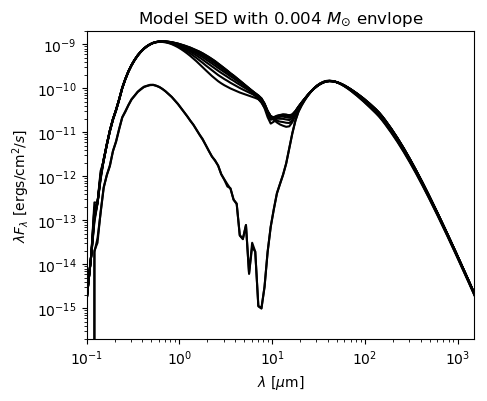
\includegraphics[width=0.45\textwidth]{model_0004_sed.png}
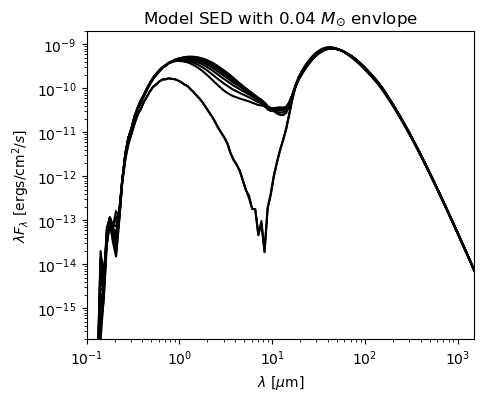
\includegraphics[width=0.45\textwidth]{model_004_sed.png}
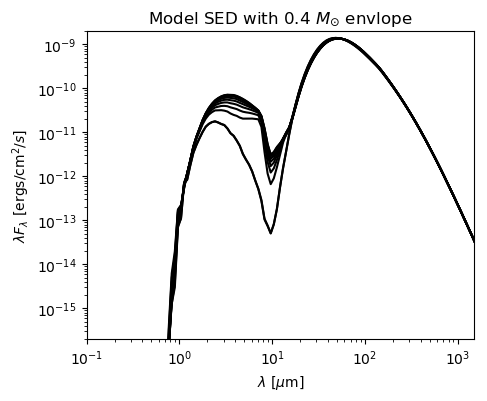
\includegraphics[width=0.45\textwidth]{model_04_sed.png}
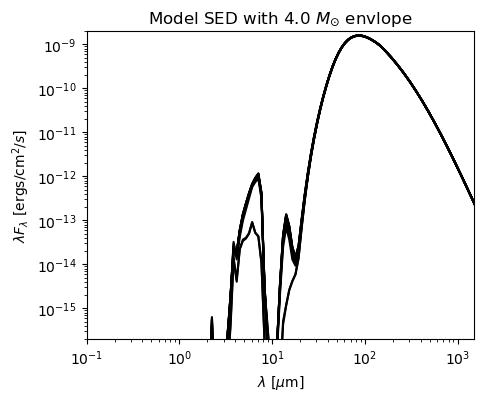
\includegraphics[width=0.45\textwidth]{model_4_sed.png}
\caption{The SEDs for the various envelope masses.}
\end{figure}
For the $0.004$ and $0.04$ \si{\msun} envelopes, we see a peak at around $0.5$ \si{\micro\meter}. From Wien's law this wavelength corresponds to a temperature of $6200$ \si{\kelvin}, so this peak corresponds to the protostar's emission. The right peak corresponds to the envelope, which produces a significant part of the emission spectrum. We note that for these lower mass envelopes, the shorter wavelength parts of the spectrum are dominated by the protostar's emission, so we don't really see the emission of the disk. Starting with the $0.4$ \si{\msun} envelope, we note that this is no longer the case, possibly because the envelope has gotten massive enough to block out the emission from the star. The left peak is now from the disk, which we can distinguish from the protostar and disk due to the difference in the wavelength corresponding to the peak. For the $4$ \si{\msun} envelope, the envelope has gotten massive enough that it starts to block out the emission from the disk as well. We note that there is a significant dip in the SED at around $10$ \si{\micro\meter}. This is explained by silicate absorption that occurs at $9.7$ \si{\micro\meter}, which becomes more evident as the envelope gets more massive.\\
\indent\hspace{1em} Here we set the viewing angles from $0\degree - 90\degree$, where $0\degree$ corresponds to a face-on view of the system and $90\degree$ an edge-on view. As we raise the value of the viewing angle, we observe less emission from the protostar and more from the disk. This is because as we increase the viewing angle, the disk begins to block out parts of the protostar, reducing the emission we receive from the protostar. By doing so we can then receive more emission from the disk as well. Here the envelope is unaffected by the viewing angle, because we can assume that the envelope is symmetric to rotation.

\item To calculate the effective temperature of the sources, we use the following equation from Krumholz:
\[\frac{\int \nu B_{\nu}(T_{bol})d\nu}{\int B_{\nu}(T_{bol})d\nu} = \frac{\int \nu F_{\nu}d\nu}{\int F_{\nu}d\nu}.\]
In practice we simply do a binary search over the temperatures until we find a value that agrees with this equation to some numerical precision. We find the following temperatures using $10000$ photons.
\begin{table}[H]
\centering
\begin{tabular}{|c|c|c|}
\hline
Mass of envelope (\si{\msun}) & Effective temperature (K) & Class \\
\hline
$0.004$ & $4650$ & III \\
$0.04$ & $1429$ & II \\
$0.4$ & $127$ & I \\
$4$ & $41$ & $0$ \\
\hline
\end{tabular}
\caption{The effective temperatures and classes of the sources for the various envelope masses.}
\end{table}
We find that these sources are in Class III, II, I, and $0$. This physically makes sense as having a more massive envelope suggests that the protostar is not as far into its evolution. 

\item We test the effects of changing the disk masses to $0.001$ \si{\msun}, $0.01$ \si{\msun}, and $1$ \si{\msun} with $0.004$ and $0.4$ \si{\msun} (not pictured) envelopes. All other values are held the same, and $10^{4}$ photons were used. We find that there is no drastic change in the effective temperature, suggesting that even with this large range in disk masses the overall emission does not change. The SEDs are also similar. These suggest that the disk doesn't contribute much to the emission of a protostellar system, and that other methods must be used when estimating the mass of the disk.

\begin{figure}[h]
\centering
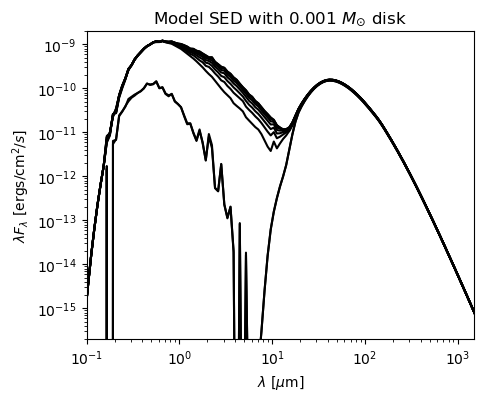
\includegraphics[width=0.45\textwidth]{model_0001_sed.png}
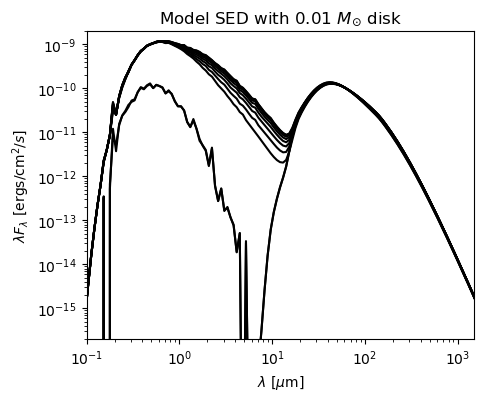
\includegraphics[width=0.45\textwidth]{model_001_sed.png}
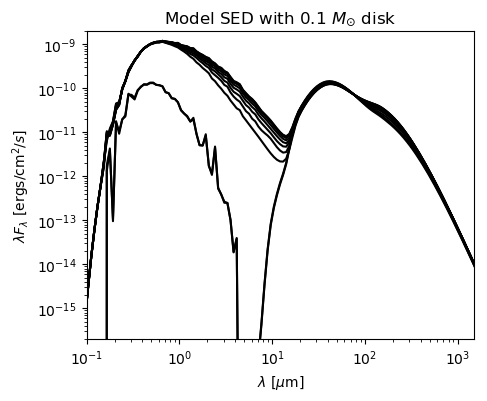
\includegraphics[width=0.45\textwidth]{model_01_sed.png}
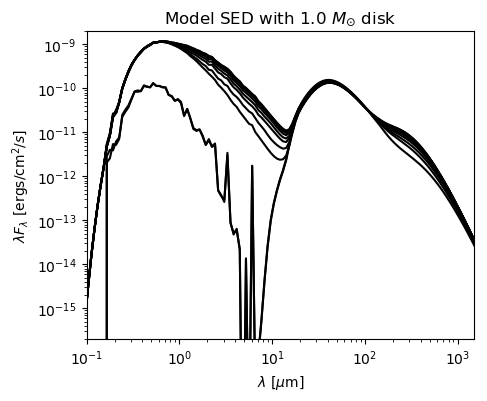
\includegraphics[width=0.45\textwidth]{model_1_sed.png}
\caption{The SEDs for the various disk masses with a $0.004$ \si{\msun} envelope.}
\end{figure}
\begin{table}[H]
\centering
\begin{tabular}{|c|c|c|}
\hline
Mass of disk (\si{\msun}) & Effective temperature (K) & Class \\
\hline
$0.001$ & $4650$ & III \\
$0.01$ & $4698$ & III \\
$0.1$ & $4650$ & III \\
$1$ & $4553$ & III \\
\hline
\end{tabular}
\caption{The effective temperatures and classes of the sources for the various disk masses with a $0.004$ \si{\msun} envelope.}
\end{table}
\end{tight_enumerate}


\end{document}